%% This is an example first chapter.  You should put chapter/appendix that you
%% write into a separate file, and add a line \include{yourfilename} to
%% main.tex, where `yourfilename.tex' is the name of the chapter/appendix file.
%% You can process specific files by typing their names in at the
%% \files=
%% prompt when you run the file main.tex through LaTeX.
\chapter{Introduction}

\section{Speech Synthesis}

Speech is most important medium of conveying opinions and expressing feeling and thoughts.
Human convert their thought into speech by using words, phrases and sentences in order to communicate with each other \cite{mumtaz2016break}. Speech is produced when air is exhaled by the lungs and vibrations are produced by air, these vibrations got a proper waveform shape by glottal cords and vocal tract. Text to Speech synthesis is the process of conversion of raw text into speech signals. It works by concatenation of small segments of recorded speech called phonemes \cite{khilari2015review}.

The TTS system comprises of two main stages. One is called Natural language Processing (NLP) and
other is called Speech Synthesis (SS). This is shown in figure \ref{fig:TTS Block Diagram}.

\begin{center}
\begin{figure}[hbtp]
\centering
  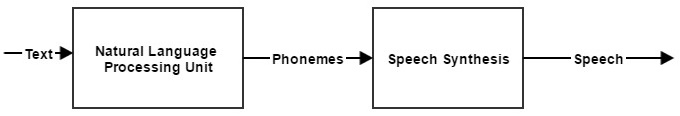
\includegraphics[width=\linewidth]{images/tts_bd.jpg}
  \caption{TTS Block Diagram}
  \label{fig:TTS Block Diagram}
\end{figure}

\end{center}

In NLP unit, text is first converted into string of letters and then word boundaries are marked by
tokenizer. This is called normalization of text. Normalized data is then converted into phonetic strings
with the help of letter to sound rules after which Syllabifier marks syllable boundaries. Sound change
rules are applied on the syllabified date. Language modeling techniques are also applied for finding
context in which a specific word is used. As human has tendency to recognize basic rules for his native
language, it is easy to judge context of a word in a sentence and what should be correct pronunciation of
that word with respect to its context. For example, it can be guessed easily that “ ”پلin a sentence is used
for ( پلmoment) or ( پلbridge) for any native speaker of Urdu. Last stage of NLP is stress intonation
marker which adds stress and intonation to the text. Speech Synthesis unit converts symbolic information
received from NLP unit into audible speech with the help of different Digital Signal Processing
Techniques. The quality of speech synthesis system is detected by naturalness and intelligibility of the speech.

Partially blinded or fully blinded people usually suffer while using computer technology when there is no assistant or 
computer is not enough interactive. Due to which text to speech systems are becoming necessity of modern life. 
These systems increase the degree to which blind people can interact with sighted 
people \cite{klatt1987review} and could boost up their hope to survive in this world 
gracefully \cite{eide2004corpus}. Many applications of speech synthesis are emerging such as 
machines that read for blinds, aids for handicaps, computers that interact with user through speech. 
For all these applications a text to
speech that convert text to speech are used \cite{klatt1982klattalk}.


In digital world there are some people who can read and understand different languages and some
who can’t understand languages except their own languages. Speech to text conversion system can
also provide a facility to exchange information between people speaking different languages \cite{khilari2015review}. TTS systems are also needed to reduce the extinction of
minority languages. As minority languages of the world are facing challenge of extinction
considerable efforts are going on from last few years for their survival. Fon language is spoken in
Republic of Benin and some other regions of Africa and it is also facing challenge of extinction \cite{dagba2014text}. The Xitsonga is spoken in more than three African countries.
TTS system of such languages will help lot of people of different literacy level \cite{baloyi2012text}.
Urdu is national language of Pakistan and it is spoken by more than 100 million people across the world \cite{top_30_languages}.
A Text-to-Speech (TTS) system for Urdu will be very helping for visually impaired, handicapped and illiterate people.

For human, the task of speech synthesis is not difficult one as they have basic knowledge of their
language but for computer some
other method has to be implemented for this task. When we talk about TTS systems speech types
and procedure for synthesis, strategies or modules used to develop systems etc. are important to
consider. Different types of speech exist such as isolated word (process single word at a time),
connected words (isolated words but separated with least gap), continuous speech (permit client
to talk while computer is processing content) and spontaneous speech (deals with variety of words
that are used rarely) as well as two types of speaker model were presented independent and
dependent of clients or speaker specifications. Vocabulary is also characterized according to size
such as small vocabulary, medium vocabulary, large vocabulary, very large vocabulary and out-of-vocabulary.
Below are the major speech generation techniques.

\section{Types of Speech Synthesis}
For the process of speech synthesis, three types of processes are used.

\subsection{Formant Synthesis}
In Formant Synthesis, simple model of speech production and set of rules are used to generate
speech. But it is very difficult to accurately describe the process of speech generation in set of
rules

\subsection{Concatenative Synthesis}
Concatenative Synthesis small units are selected from carrier sentences which then join to form
speech of complete sentence. These small units are called phonemes. These are the units which
collectively describe correct pronunciation of a word. This process is easy as compared to previous one
as number of such phonemes is limited for any language. For English, there are 44 such phonemes.
Similarly in Urdu, there are 44 consonants, 8 long vowels, 7 long nasal vowels, 3 short vowels and many
diphthongs \cite{saleem2002urdu}. This reduce distortion but it can decrease the naturalness.
That’s why the derived synthetic speech may not resemble the donor speaker in training database \cite{huang1996whistler}.

\subsection{Statistical Parametric Speech Synthesis}
Statistical parametric speech synthesis is another approach which uses parameters to describe
speech. In this technique, model is learned from speech data. This technique works better than
concatenative technique \cite{merritt2013investigating}. 

\section{Quality}
The intelligibility and naturalness is the measure of quality of the synthesized speech \cite{swetha2013text}. 
There is lots of experimentation over naturalness of voice as a result of TTS
systems. In today’s world different segments are recorded and then concatenated for completing a
message. A collection of speech words is collected and maintained in database by using a reader
who reads large series of text. In these kind of system, to maintain the consistency the speaker
speaks in a single style and keep in mind the distance from microphone and other factors to avoid
the inconsistency. This type of TTS system is not required at all as the need is to have a system
which can be expressive and convey message with proper expressions and styles. Work is
performed to build a system that can convey the message according to the needs of the users. A
single style of communication can lead towards wrong messages and can cause other problems of
understandings. For example, it is not appropriate to convey a good news and bad news in a same
style and manner. Similarly, it is not acceptable to ask a question in neutral way of communication \cite{eide2004corpus}.
Multiple techniques like linear regression and neural networks were applied
to get the results with improvements. Concatenation techniques are applied to get fully
expressive and stylish messages for end users. By using concatenation technique users can
customize and add styles and expression through provided Speech Synthesis Markup Language (SSML) \cite{eide2004corpus}. 
Timing of events in speech is also important as timing of events in
speech signals are affected by some contextual factors like phone identity factors. These factors
make it difficult to control timing of events \cite{tokuda2000speech}. There are some approaches which have been proposed
to control timing of events like linear regression \cite{kaiki1992linguistic} and tree regression \cite{riley1992tree}. 
A new technique is proposed in \cite{tokuda2000speech} in which timing of events is
controlled by multi-dimensional Gaussian distribution based Hidden Markov model.

\section{Architecture}
Text to speech is a way of communication and transferring information using words and styles of
speaking \cite{eide2004corpus}. It has two processes which are text processing and speech
generation. In text processing given input text is processed so that to get appropriate chain of
phonemic units. Speech generator takes these units as inputs and convert them into synthetic
speech by selection of a unit from large corpus TTS system for small database is easier to
implement but not in good quality \cite{black2007statistical} \cite{zen2007hmm} \cite{raj2007text}.
Different researchers and developers use different strategies to develop TTS system such as in \cite{kabir2002natural}, 
author interpret text to speech system as, it converts raw text into intelligible speech signals
by following two sub processes called High-level synthesis and Low-level synthesis. High-level
synthesis converts text into phonetic strings and Low-level synthesis converts these strings into
speech signals \cite{kabir2002natural}. In \cite{hussain2005phonological}, TTS system is divided in three modules.

\begin{enumerate}
  \item Natural language Processing
  \item Text Parameterization
  \item Speech Synthesis
\end{itemize}
Natural Language processing unit converts text into phonetic strings. The second and
third stages use these phonetic strings and convert them into speech signals. This is shown in figure \ref{fig:Architecture of TTS}.
\begin{center}
\begin{figure}[hbtp]
\centering
  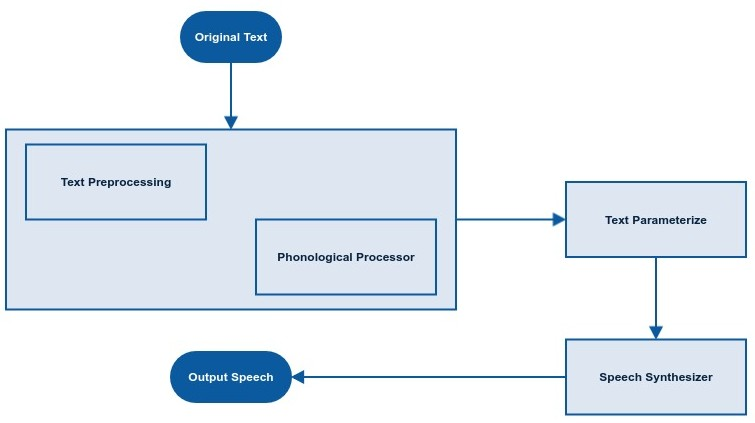
\includegraphics[width=\linewidth]{images/flow_chart.jpg}
  \caption{Architecture of TTS}
  \label{fig:Architecture of TTS}
\end{figure}
\end{center}
In \cite{liberman1992text}, TTS system is implemented by following four modules in
sequence.

\begin{enumerate}
  \item Text Analysis
  \item Word Pronunciation
  \item Phonetic Interpretation
  \item Speech Signal Generation
\end{itemize}

In text analysis, the inputted text is segmented into sentences and later on to words.
These words are then categorized according to their syntactic and contextual meaning. The
numbers and abbreviations are also processed in this step. In word pronunciation process, words
are represented by respective phonetic notations by using word pronunciation dictionary. In
phonetic interpretation the duration of phonetic segments, pitch, accents are assigned. Signal
generation component of TTS system takes output from all above processes and generate a signal
of speech using a function. In \cite{urdu_text_preprocessing}, text-to-Speech system is divided in
two parts. One is called Natural Language Processing unit and other is called Speech Synthesis
unit. Natural Language Processing unit preprocess text and converts it into phonetic strings. These
phonetic strings are then marked by stress marker and passed to speech synthesis unit which
converts it into speech signals.


% Text to speech system provides a range of applications from talking toys to unrestricted text to
% speech system; these systems make ways and possibilities for information displays \cite{carlson1976text}.
%
% Micro-optimization is a technique to reduce the overall operation count of
% floating point operations.  In a standard floating point unit, floating
% point operations are fairly high level, such as ``multiply'' and ``add'';
% in a micro floating point unit ($\mu$FPU), these have been broken down into
% their constituent low-level floating point operations on the mantissas and
% exponents of the floating point numbers.
%
% Chapter two describes the architecture of the $\mu$FPU unit, and the
% motivations for the design decisions made.
%
% Chapter three describes the design of the compiler, as well as how the
% optimizations discussed in section~\ref{ch1:opts} were implemented.
%
% Chapter four describes the purpose of test code that was compiled, and which
% statistics were gathered by running it through the simulator.  The purpose
% is to measure what effect the micro-optimizations had, compared to
% unoptimized code.  Possible future expansions to the project are also
% discussed.
%
% \section{Motivations for micro-optimization}
%
% The idea of micro-optimization is motivated by the recent trends in computer
% architecture towards low-level parallelism and small, pipelineable
% instruction sets \cite{patterson:risc,rad83}.  By getting rid of more
% complex instructions and concentrating on optimizing frequently used
% instructions, substantial increases in performance were realized.
%
% Another important motivation was the trend towards placing more of the
% burden of performance on the compiler.  Many of the new architectures depend
% on an intelligent, optimizing compiler in order to realize anywhere near
% their peak performance
% \cite{ellis:bulldog,pet87,coutant:precision-compilers}.  In these cases, the
% compiler not only is responsible for faithfully generating native code to
% match the source language, but also must be aware of instruction latencies,
% delayed branches, pipeline stages, and a multitude of other factors in order
% to generate fast code \cite{gib86}.
%
% Taking these ideas one step further, it seems that the floating point
% operations that are normally single, large instructions can be further broken
% down into smaller, simpler, faster instructions, with more control in the
% compiler and less in the hardware.  This is the idea behind a
% micro-optimizing FPU; break the floating point instructions down into their
% basic components and use a small, fast implementation, with a large part of
% the burden of hardware allocation and optimization shifted towards
% compile-time.
%
% Along with the hardware speedups possible by using a $\mu$FPU, there are
% also optimizations that the compiler can perform on the code that is
% generated.  In a normal sequence of floating point operations, there are
% many hidden redundancies that can be eliminated by allowing the compiler to
% control the floating point operations down to their lowest level.  These
% optimizations are described in detail in section~\ref{ch1:opts}.
%
% \section{Description of micro-optimization}\label{ch1:opts}
%
% In order to perform a sequence of floating point operations, a normal FPU
% performs many redundant internal shifts and normalizations in the process of
% performing a sequence of operations.  However, if a compiler can
% decompose the floating point operations it needs down to the lowest level,
% it then can optimize away many of these redundant operations.
%
% If there is some additional hardware support specifically for
% micro-optimization, there are additional optimizations that can be
% performed.  This hardware support entails extra ``guard bits'' on the
% standard floating point formats, to allow several unnormalized operations to
% be performed in a row without the loss information\footnote{A description of
% the floating point format used is shown in figures~\ref{exponent-format}
% and~\ref{mantissa-format}.}.  A discussion of the mathematics behind
% unnormalized arithmetic is in appendix~\ref{unnorm-math}.
%
% The optimizations that the compiler can perform fall into several categories:
%
% \subsection{Post Multiply Normalization}
%
% When more than two multiplications are performed in a row, the intermediate
% normalization of the results between multiplications can be eliminated.
% This is because with each multiplication, the mantissa can become
% denormalized by at most one bit.  If there are guard bits on the mantissas
% to prevent bits from ``falling off'' the end during multiplications, the
% normalization can be postponed until after a sequence of several
% multiplies\footnote{Using unnormalized numbers for math is not a new idea; a
% good example of it is the Control Data CDC 6600, designed by Seymour Cray.
% \cite{thornton:cdc6600} The CDC 6600 had all of its instructions performing
% unnormalized arithmetic, with a separate {\tt NORMALIZE} instruction.}.
%
% % This is an example of how you would use tgrind to include an example
% % of source code; it is commented out in this template since the code
% % example file does not exist.  To use it, you need to remove the '%' on the
% % beginning of the line, and insert your own information in the call.
% %
% %\tagrind[htbp]{code/pmn.s.tex}{Post Multiply Normalization}{opt:pmn}
%
% As you can see, the intermediate results can be multiplied together, with no
% need for intermediate normalizations due to the guard bit.  It is only at
% the end of the operation that the normalization must be performed, in order
% to get it into a format suitable for storing in memory\footnote{Note that
% for purposed of clarity, the pipeline delays were considered to be 0, and
% the branches were not delayed.}.
%
% \subsection{Block Exponent}
%
% In a unoptimized sequence of additions, the sequence of operations is as
% follows for each pair of numbers ($m_1$,$e_1$) and ($m_2$,$e_2$).
% \begin{enumerate}
%   \item Compare $e_1$ and $e_2$.
%   \item Shift the mantissa associated with the smaller exponent $|e_1-e_2|$
%         places to the right.
%   \item Add $m_1$ and $m_2$.
%   \item Find the first one in the resulting mantissa.
%   \item Shift the resulting mantissa so that normalized
%   \item Adjust the exponent accordingly.
% \end{enumerate}
%
% Out of 6 steps, only one is the actual addition, and the rest are involved
% in aligning the mantissas prior to the add, and then normalizing the result
% afterward.  In the block exponent optimization, the largest mantissa is
% found to start with, and all the mantissa's shifted before any additions
% take place.  Once the mantissas have been shifted, the additions can take
% place one after another\footnote{This requires that for n consecutive
% additions, there are $\log_{2}n$ high guard bits to prevent overflow.  In
% the $\mu$FPU, there are 3 guard bits, making up to 8 consecutive additions
% possible.}.  An example of the Block Exponent optimization on the expression
% X = A + B + C is given in figure~\ref{opt:be}.
%
% % This is an example of how you would use tgrind to include an example
% % of source code; it is commented out in this template since the code
% % example file does not exist.  To use it, you need to remove the '%' on the
% % beginning of the line, and insert your own information in the call.
% %
% %\tgrind[htbp]{code/be.s.tex}{Block Exponent}{opt:be}
%
% \section{Integer optimizations}
%
% As well as the floating point optimizations described above, there are
% also integer optimizations that can be used in the $\mu$FPU.  In concert
% with the floating point optimizations, these can provide a significant
% speedup.
%
% \subsection{Conversion to fixed point}
%
% Integer operations are much faster than floating point operations; if it is
% possible to replace floating point operations with fixed point operations,
% this would provide a significant increase in speed.
%
% This conversion can either take place automatically or or based on a
% specific request from the programmer.  To do this automatically, the
% compiler must either be very smart, or play fast and loose with the accuracy
% and precision of the programmer's variables.  To be ``smart'', the computer
% must track the ranges of all the floating point variables through the
% program, and then see if there are any potential candidates for conversion
% to floating point.  This technique is discussed further in
% section~\ref{range-tracking}, where it was implemented.
%
% The other way to do this is to rely on specific hints from the programmer
% that a certain value will only assume a specific range, and that only a
% specific precision is desired.  This is somewhat more taxing on the
% programmer, in that he has to know the ranges that his values will take at
% declaration time (something normally abstracted away), but it does provide
% the opportunity for fine-tuning already working code.
%
% Potential applications of this would be simulation programs, where the
% variable represents some physical quantity; the constraints of the physical
% system may provide bounds on the range the variable can take.
% \subsection{Small Constant Multiplications}
%
% One other class of optimizations that can be done is to replace
% multiplications by small integer constants into some combination of
% additions and shifts.  Addition and shifting can be significantly faster
% than multiplication.  This is done by using some combination of
% \begin{eqnarray*}
% a_i & = & a_j + a_k \\
% a_i & = & 2a_j + a_k \\
% a_i & = & 4a_j + a_k \\
% a_i & = & 8a_j + a_k \\
% a_i & = & a_j - a_k \\
% a_i & = & a_j \ll m \mbox{shift}
% \end{eqnarray*}
% instead of the multiplication.  For example, to multiply $s$ by 10 and store
% the result in $r$, you could use:
% \begin{eqnarray*}
% r & = & 4s + s\\
% r & = & r + r
% \end{eqnarray*}
% Or by 59:
% \begin{eqnarray*}
% t & = & 2s + s \\
% r & = & 2t + s \\
% r & = & 8r + t
% \end{eqnarray*}
% Similar combinations can be found for almost all of the smaller
% integers\footnote{This optimization is only an ``optimization'', of course,
% when the amount of time spent on the shifts and adds is less than the time
% that would be spent doing the multiplication.  Since the time costs of these
% operations are known to the compiler in order for it to do scheduling, it is
% easy for the compiler to determine when this optimization is worth using.}.
% \cite{magenheimer:precision}
%
% \section{Other optimizations}
%
% \subsection{Low-level parallelism}
%
% The current trend is towards duplicating hardware at the lowest level to
% provide parallelism\footnote{This can been seen in the i860; floating point
% additions and multiplications can proceed at the same time, and the RISC
% core be moving data in and out of the floating point registers and providing
% flow control at the same time the floating point units are active. \cite{byte:i860}}
%
% Conceptually, it is easy to take advantage to low-level parallelism in the
% instruction stream by simply adding more functional units to the $\mu$FPU,
% widening the instruction word to control them, and then scheduling as many
% operations to take place at one time as possible.
%
% However, simply adding more functional units can only be done so many times;
% there is only a limited amount of parallelism directly available in the
% instruction stream, and without it, much of the extra resources will go to
% waste.  One process used to make more instructions potentially schedulable
% at any given time is ``trace scheduling''.  This technique originated in the
% Bulldog compiler for the original VLIW machine, the ELI-512.
% \cite{ellis:bulldog,colwell:vliw}  In trace scheduling, code can be
% scheduled through many basic blocks at one time, following a single
% potential ``trace'' of program execution.  In this way, instructions that
% {\em might\/} be executed depending on a conditional branch further down in
% the instruction stream are scheduled, allowing an increase in the potential
% parallelism.  To account for the cases where the expected branch wasn't
% taken, correction code is inserted after the branches to undo the effects of
% any prematurely executed instructions.
%
% \subsection{Pipeline optimizations}
%
% In addition to having operations going on in parallel across functional
% units, it is also typical to have several operations in various stages of
% completion in each unit.  This pipelining allows the throughput of the
% functional units to be increased, with no increase in latency.
%
% There are several ways pipelined operations can be optimized.  On the
% hardware side, support can be added to allow data to be recirculated back
% into the beginning of the pipeline from the end, saving a trip through the
% registers.  On the software side, the compiler can utilize several tricks to
% try to fill up as many of the pipeline delay slots as possible, as
% seendescribed by Gibbons. \cite{gib86}
